\documentclass[aspectratio=169, xcolor=dvipsnames]{beamer}
\hypersetup{pdfpagemode=FullScreen}
\beamertemplatenavigationsymbolsempty
\setbeamertemplate{caption}{\raggedright\insertcaption\par}
\usepackage[utf8]{inputenc}
\usepackage[spanish]{babel}
\usepackage{circuitikz}
\usepackage{siunitx}
\usepackage{graphicx}
\usepackage{xcolor}
\usepackage{amsmath} 
\usepackage{esint}
\usepackage{biblatex}
\usepackage{minted}
\usepackage[T1]{fontenc}
\usepackage{lmodern}
\usepackage{listings}
\usepackage{multicol}

\definecolor{mygreen}{rgb}{0,0.6,0}
\lstdefinestyle{mystyle}{
    commentstyle=\color{mygreen},
    keywordstyle=\color{blue},
}
\lstset{style=mystyle}

\definecolor{myblue}{rgb}{0.29, 0.5, 0.94}

\title{Sistemas Operativos de Propósito General}
\subtitle{Introducción a Linux}
\author[Laboratorio de Sistemas Embebidos]{
\includegraphics[scale=0.15]{resources/images/utn_logo.png}}
\institute{UTN FRA\\Departamento de Ingeniería Electrónica\\Técnicas Digitales III}
\date[]{Septiembre 2024} 
\usetheme{Warsaw}
\usecolortheme[named=myblue]{structure}
\setbeamertemplate{headline}{}

\begin{document}

\frame{\titlepage}
\begin{frame}{Introducción a Linux}{Índice}
\begin{multicols}{2}
\tableofcontents
\end{multicols}
\end{frame}

\section{Proyecto GNU/Linux}
\subsection{Historia de Linux}
\begin{frame}{Introducción a Linux}{Proyecto GNU/Linux}
\begin{columns}
\begin{column}{0.5\textwidth}
\begin{itemize}
    \item 1983 Richard Stallman arranca el proyecto GNU.
    \item Surge la licencia GNU GPL.
    \item 1991 Linus Torvalds desarrolla el kernel de Linux.
    \item 1992 se licencia Linux bajo GNU GPL.
\end{itemize}
\end{column}
\begin{column}{0.5\textwidth}
\begin{multicols}{2}
\begin{figure}
    \centering
    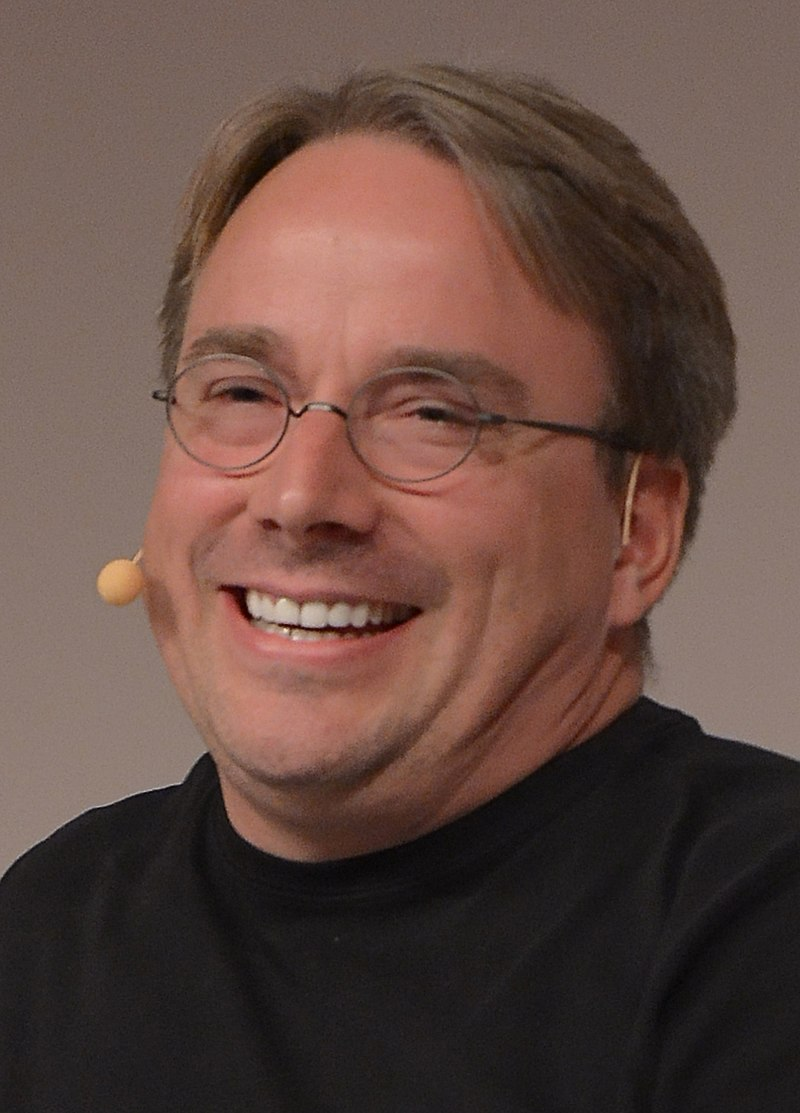
\includegraphics[width=1\linewidth]{resources/images/linus_torvalds.jpg}
    \caption{Linus Torvalds}
\end{figure}
\begin{figure}
    \centering
    
\includegraphics[width=1\linewidth]{resources/images/richard_stallman.jpg}
    \caption{Richard Stallman}
\end{figure}
\end{multicols}
\end{column}
\end{columns}
\end{frame}

\subsection{Pros de Linux}
\begin{frame}{Introducción a Linux}{Pros de Linux}
Entre algunas ventajas y razones para elegir Linux como sistema operativo podemos mencionar:\newline

\begin{itemize}
    \item Es Open Source.
    \item Mucha customización.
    \item Distribuciones para todas las necesidades.
    \item Corre en casi cualquier cosa.
    \item Es gratis!
\end{itemize}
    
\end{frame}

\subsection{El kernel de Linux}
\begin{frame}{Introducción a Linux}{El kernel de Linux}
\begin{figure}
    \centering
    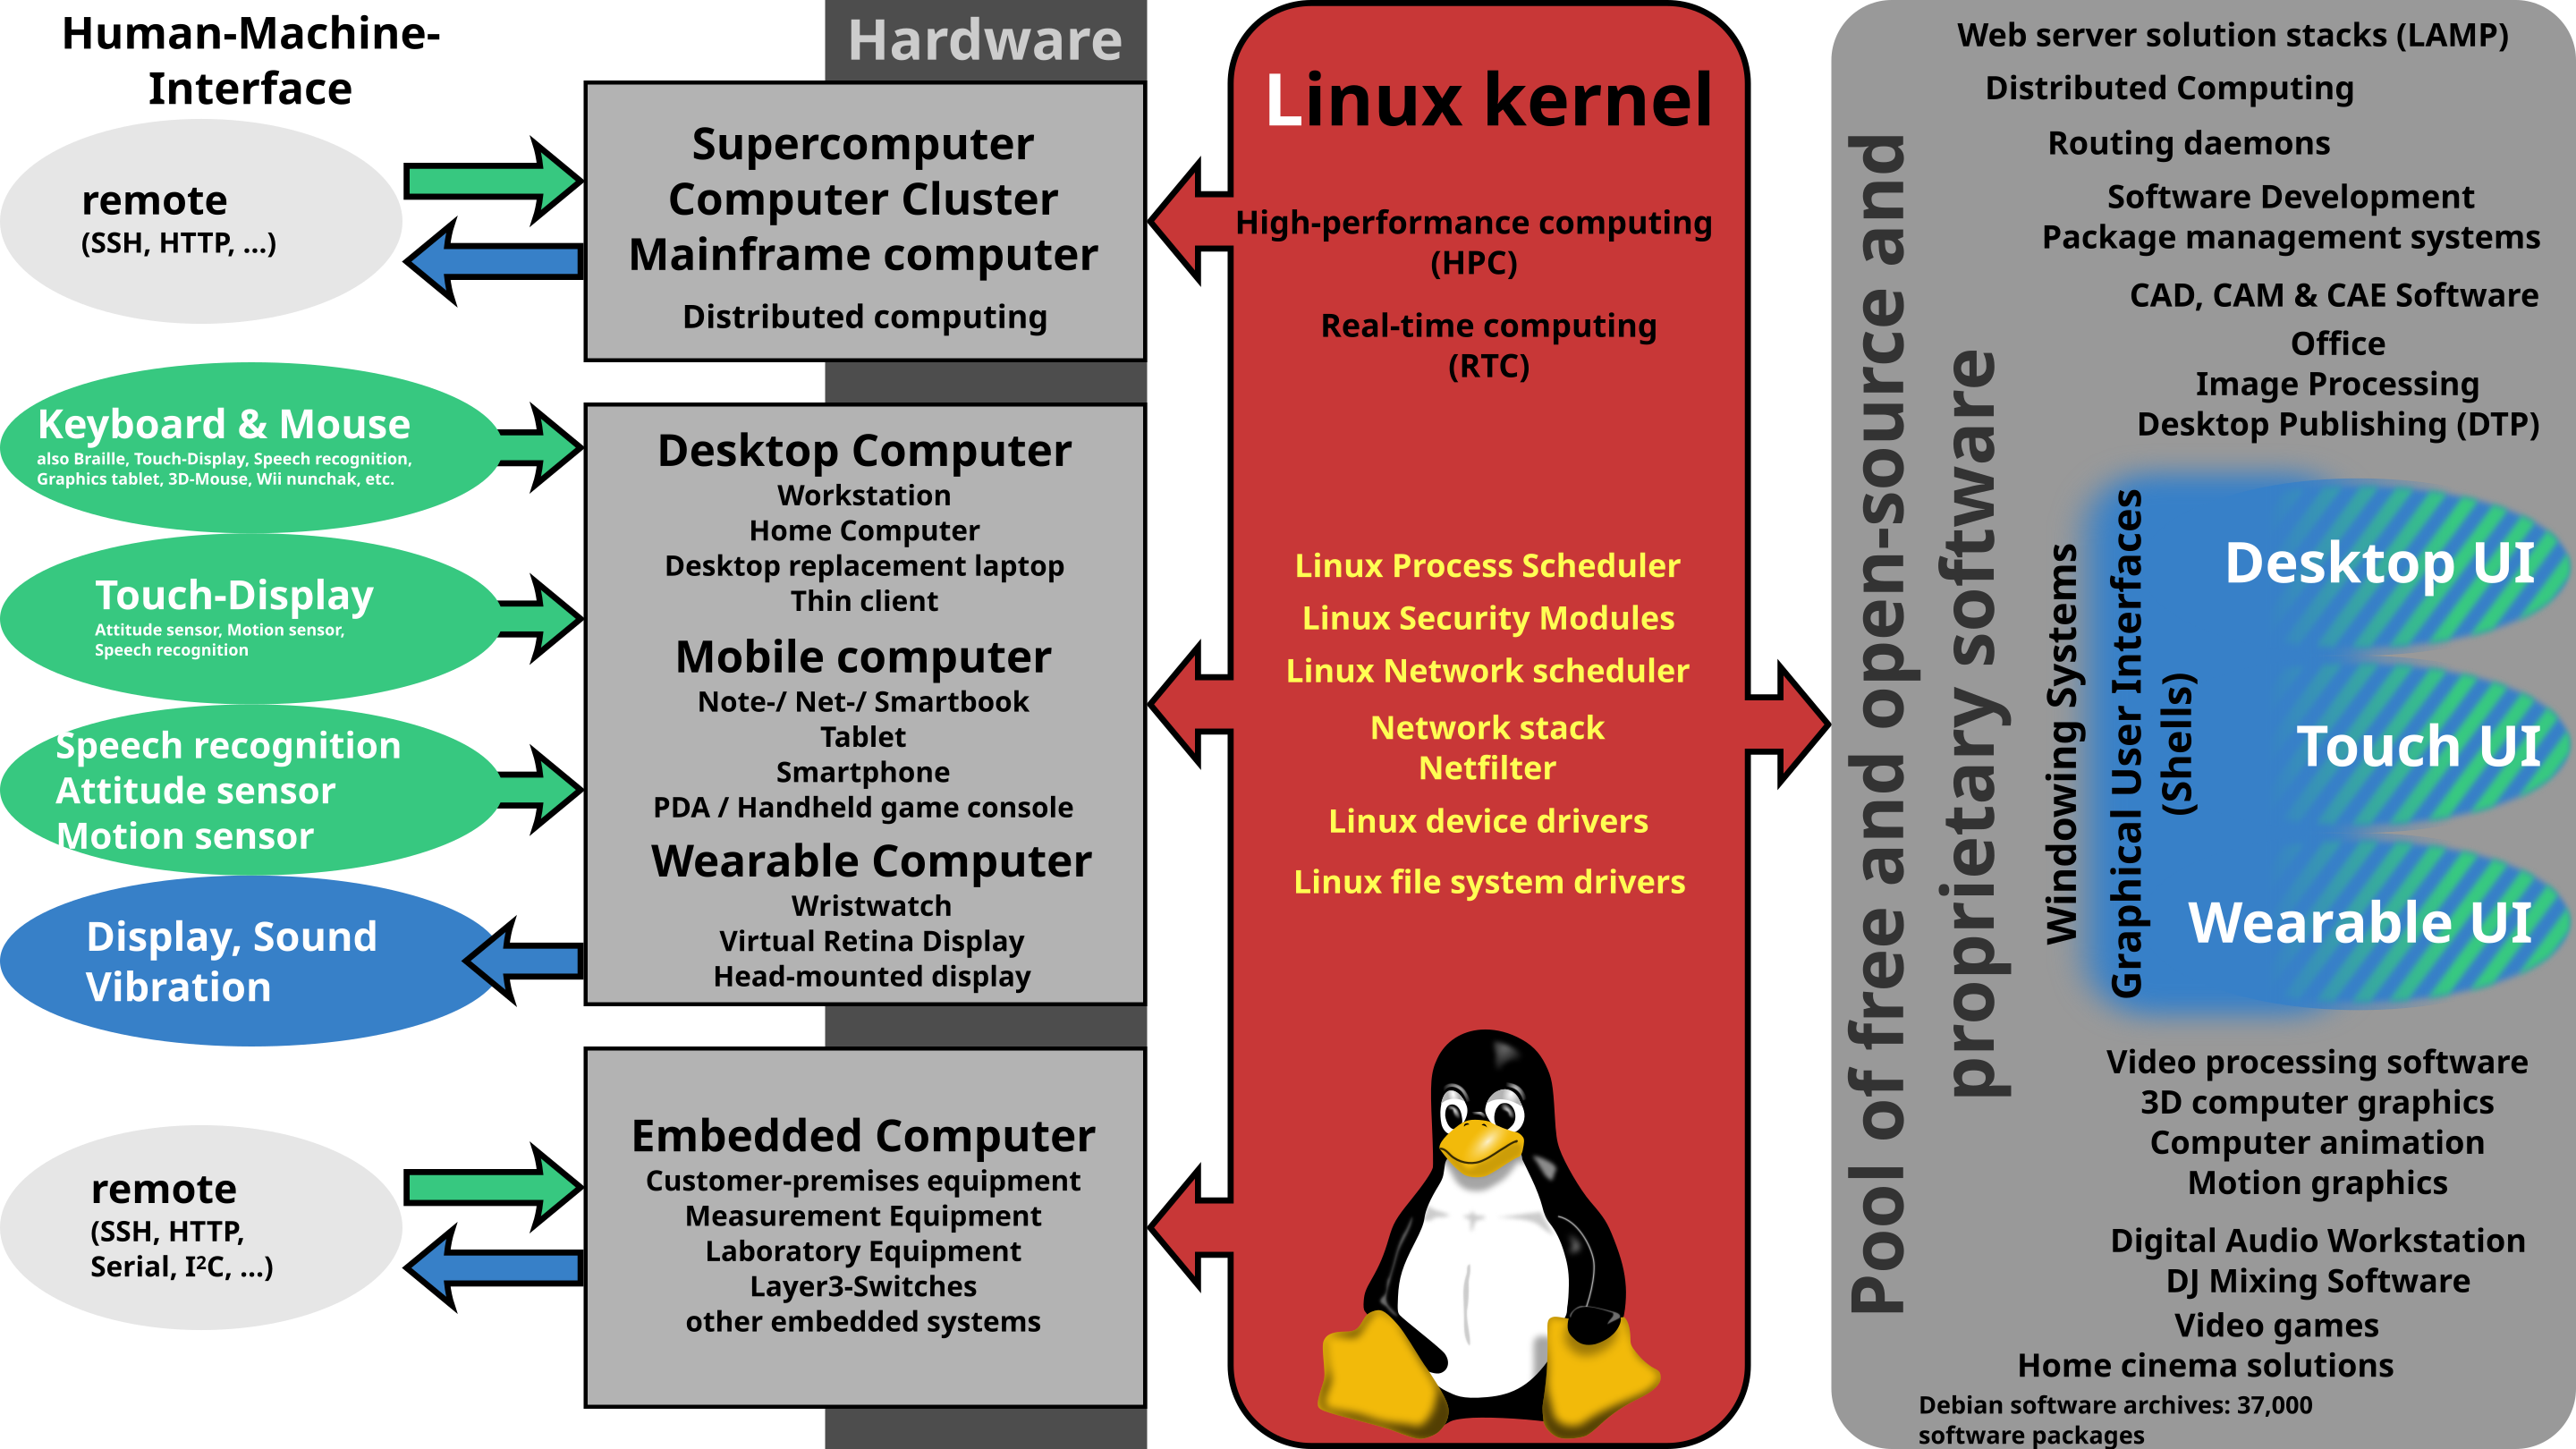
\includegraphics[width=0.9\linewidth]{resources/images/linux_kernel.svg.png}
\end{figure}
\end{frame}

\subsection{Distribuciones}
\begin{frame}{Introducción a Linux}{Distribuciones}
Que es una distribución o distro?\newline
\begin{center}
distro = Linux Kernel + Bibliotecas GNU + Software Específico
\end{center}
Hay distros para todos los gustos y necesidades. \textcolor{myblue}{\href{https://upload.wikimedia.org/wikipedia/commons/a/ad/2023_Linux_Distributions_Timeline.svg}{Acá}} hay una lista completa. Algunas de las más populares mencionamos abajo.
\begin{multicols}{5}
\begin{figure}
    \centering
    \href{https://ubuntu.com/desktop}{
\includegraphics[width=0.5\linewidth]{resources/images/ubuntu_logo.png}}
    \caption{Ubuntu}
\end{figure}
\begin{figure}
    \centering
    \href{https://www.debian.org}{
\includegraphics[width=0.5\linewidth]{resources/images/debian_logo.png}}
    \caption{Debian}
\end{figure}
\begin{figure}
    \centering
    \href{https://linuxmint.com}{
\includegraphics[width=0.5\linewidth]{resources/images/mint_logo.png}}
    \caption{Linux Mint}
\end{figure}
\begin{figure}
    \centering
    \href{https://archlinux.org}{
\includegraphics[width=0.5\linewidth]{resources/images/arch_logo.png}}
    \caption{Arch Linux}
\end{figure}
\begin{figure}
    \centering
    \href{https://zorin.com/os/}{
\includegraphics[width=0.5\linewidth]{resources/images/zorin_logo.png}}
    \caption{Zorin}
\end{figure}
\end{multicols}
\end{frame}

\section{Distro de la Cátedra}
\subsection{Software y OS}
\begin{frame}{Introducción a Linux}{Distro para la Cátedra}
Para la cátedra, vamos a usar una distro de Raspbian corriendo en una máquina virtual para poder practicar y resolver ejercicios. 
Existe una versión de Raspbian preparada para computadoras con procesadores Intel y AMD.
\newline
\begin{columns}
\begin{column}{0.25\textwidth}
\begin{figure}
    \centering
    \href{https://www.virtualbox.org}{
\includegraphics[width=0.5\linewidth]{resources/images/virtualbox_logo.png}}
    \caption{Oracle Virtual Box}
\end{figure}
\end{column}
\begin{column}{0.25\textwidth}
\begin{figure}
    \centering
    \href{https://www.raspberrypi.com/software/raspberry-pi-desktop/}{
\includegraphics[width=0.5\linewidth]{resources/images/rapsbian_logo.png}}
    \caption{Raspberry Pi Desktop}
\end{figure}
\end{column}
\end{columns}
\end{frame}

\subsection{Requisitos del sistema}
\begin{frame}{Introducción a Linux}{Recursos Mínimos para Raspberry Pi Desktop}
En la configuración de Virual Box, tenemos que elegir el hardware reservado para nuestra máquina virtual. Entrando a configuración avanzada, elegimos:
\newline
\begin{itemize}
    \item Debian de 32 bits
    \item 2048 MB (2 GB) de RAM
    \item Dos CPUs
    \item 20 GB de almacenamiento dinámico
\end{itemize}
\end{frame}

\subsection{Instalación del OS}
\begin{frame}{Introducción a Linux}{Instalación de Raspberry Pi Desktop}
Corremos la máquina virtual y elegimos la opción de instalar. Entre los pasos de instalción elegimos:
\newline
\begin{itemize}
    \item Teclado
    \item Elegimos usar disco entero en las particiones
    \item Dejamos que la instalación finalice y agregamos el GRUB boot loader
    \item Dejar que el sistema se reinicie y terminar la configuración
\end{itemize}
\end{frame}

\subsection{Paquetes requeridos}
\begin{frame}{Introducción a Linux}{Instalación de paquetes necesarios}
Para asegurarnos de que tengamos todo lo necesario para trabajar, vamos a correr:
\newline
\begin{enumerate}
    \item sudo apt-get update -y
    \item sudo apt-get upgrade -y
    \item sudo apt install build-essential bc bison flex libncurses5-dev libssl-dev -y
    \item sudo apt install raspberrypi-kernel-headers -y
\end{enumerate}
\end{frame}

\section{Raspberry Pi 4}
\subsection{Especificaciones}
\begin{frame}{Introducción a Linux}{Raspberry Pi 4}
\begin{columns}
\begin{column}{0.6\textwidth}
\begin{figure}
    \centering
    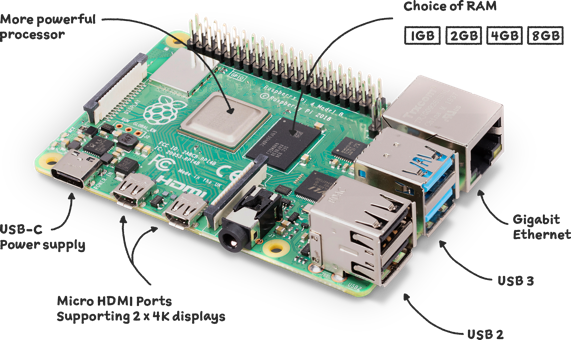
\includegraphics[width=0.9\linewidth]{resources/images/raspberry_pi_4.png}
\end{figure}
\end{column}
\begin{column}{0.4\textwidth}
\begin{itemize}
    \item Quad core Cortex-A72 (ARM v8) 64-bit SoC @ 1.8GHz
    \item 1GB, 2GB, 4GB u 8GB de RAM
    \item Comunicación wireless de 2.4GHz y 5GHz
    \item GPIO de 40 pines con periféricos varios
    \item Dos salidas mini HDMI a 4K
    \item Alimentación por USB-C de 5V@3A
\end{itemize}
\end{column}
\end{columns}
\end{frame}

\subsection{Conexión remota}
\begin{frame}{Introducción a Linux}{Conexión remota}
Las Raspberry Pi 4 del laboratorio se encuentran conectadas a la red de UTN\_2022. Con una PC conectada a la misma red podemos conectarnos remotamente por un cliente de SSH como \textcolor{myblue}{\href{https://www.putty.org}{PuTTY}} o \textcolor{myblue}{\href{https://termius.com}{Termius}}.
Una vez que tengamos nuestro cliente SSH, entramos a la Raspberry Pi 4 como:
\newline
\begin{center}
    lse@lse-pi4-01.local
\end{center}
Donde:
\begin{itemize}
    \item \textbf{lse} es el usuario con el que vamos a ingresar
    \item \textbf{lse-pi4-01} es el \textit{hostname}
    \item \textbf{.local} sirve para indicar que este hostname vive en la misma red de nuestra PC
\end{itemize}
Si la conexión se establece, entramos a la Raspberry Pi con la contraseña \textit{lse}.
\end{frame}

\section{Bibliografía de Consulta}
\begin{frame}[containsverbatim]{Introducción a Linux}{Bibliografía de Consulta}
\begin{itemize}
\begin{multicols}{2}
    \item \href{https://es.wikipedia.org/wiki/Historia_de_Linux}{Historia de Linux}
    \item \href{https://www.synopsys.com/glossary/what-is-open-source-software.html#:~:text=can%20Synopsys%20help%3F-,Definition,distribution%20with%20its%20original%20rights.}{Qué es el Software de Código Abierto}
    \item \href{https://www.gnu.org/licenses/gpl-3.0.en.html}{GNU General Public License}
    \item \href{https://www.redhat.com/en/topics/linux/what-is-the-linux-kernel}{Qué es el kernel de Linux}
    \item \href{https://github.com/torvalds/linux}{Código fuente del kernel de Linux}
    \item \href{https://docs.kernel.org}{Documentación del kernel de Linux}
    \item \href{https://www.raspberrypi.com/products/raspberry-pi-4-model-b/specifications/}{Especificaciones de la Raspberry Pi 4}
    \item \href{https://www.ssh.com/academy/ssh/client}{Clientes SSH}
\end{multicols}
\end{itemize}
\end{frame}

\end{document}
